\documentclass{beamer}
\usepackage[utf8]{inputenc}
\usepackage{graphicx}

\hypersetup{
    colorlinks,%
    citecolor=blue,%
    filecolor=blue,%
    linkcolor=blue,%
    urlcolor=blue 
    %urlcolor=mygreylink     % can put red here to better visualize the links
}

\author[Sowmya Vajjala]{Instructor: Sowmya Vajjala}

\title[LING 520]{LING 520: Computational Analysis of English}
\subtitle{Semester: FALL '16}

\date{18 October 2016}

\institute{Iowa State University, USA}
%%%%%%%%%%%%%%%%%%%%%%%%%%%

\begin{document}

\begin{frame}\titlepage
\end{frame}

\begin{frame}
\frametitle{Class Outline}
\begin{itemize}
\item Assignment 3 Discussion
\item Text Classification: last week Recap 
\item Brief overview of some more classification algorithms%  Logistic Regression, Decision trees, Random Forests, Support Vector Machines
\item Assignment 4 Description
\end{itemize}
\end{frame}

\begin{frame}
\frametitle{}
\Large Assignment 3 Discussion
\end{frame} %20min

\begin{frame}
\frametitle{}
\Large Text Classification - last week Recap 
\end{frame} %20min

\begin{frame}
\frametitle{What is text classification?}
\begin{itemize}
\item Assuming we have some example texts which have some pre-defined class/category labels,
\item text classification has this goal: developing a "model" of categorization based these example texts (training data)
\item ... and using this model to assign categories to new texts.
\end{itemize}
Note: J\&M 3rd Edition draft chapters on Jurafksy's website has a good chapter on Text Classification. Please read. \url{https://web.stanford.edu/~jurafsky/slp3/7.pdf}
\end{frame}

\begin{frame}
\frametitle{Text Classification - Process}
\begin{itemize}
\item Step 1: You have some collection of texts labeled with some categories, which you will use as training data for your model \pause
\item Step 2: You design some features that you think can distinguish between these categories (kitchen sink strategy or hand-crafted) \pause
\item Step 3: Convert those texts into feature vectors. \pause
\item Step 4: Develop or use an existing learning algorithm that can learn a classification function based on the values of all these features for the texts \pause
\item Step 5: Evaluate the classification based on some measure. Tune your classifier with better features, better learning algorithm or with more data (or all of those) \pause
\item Step 6: Stop when you are satisfied, and deploy your classifier in some real world application \pause \\ (and discover all that research still does not result in material benefit!)
\end{itemize}
\end{frame}

\begin{frame}
\frametitle{Measuring Success}
Multiple ways. Depends on the nature of your dataset, and your application.
\begin{itemize}
\item Prediction accuracy on test set: typically used in most ML evaluation for text, images, videos, all sorts of things
\item False positive rate (Type 1 Error), False negatives (Type 2 error) - typically in medical applications
\item Precision (TP/(TP+FP)), Recall (TP/(TP+FN)), F-score (2PR/(P+R)) - typically in information retrieval, text classification
\item Revenue increase - in e-commerce applications
\end{itemize}
\end{frame}

\begin{frame}
\frametitle{Some commonly used features in text classification}
\begin{itemize}
\item ngrams (word, character, POS, mixed representations)
\item specific hand-crafted features: e.g., number of spelling errors, number of dependent clauses per clause, number of preposition phrases per sentence etc.
\item feature representation: binary (presence or absence), count (number of occurrences), ratios etc.
\end{itemize}
\end{frame}

\begin{frame}
\frametitle{Some commonly used learning algorithms}
\begin{itemize}
\item \textbf{Naive bayes classifier}
\item \textbf{K-nearest neighbors classifier}
\item Logistic regression
\item Decision Trees and Random forests
\item Support vector machines, neural network classifiers
\end{itemize}
.. etc. Note: I will only give an overview of how these work, to give an intuitive idea. Details are found in machine learning classes or textbooks. 
\end{frame}

\begin{frame}
\frametitle{} %15min
\Large Logistic Regression
\end{frame}

\begin{frame}
\frametitle{Logistic Regression}
\begin{itemize}
\item Goal: same as any other classification algorithm. Classify a given text into one of the pre-defined categories, based on some feature representation.
\item Difference compared to naive bayes or knn: learning function.
\item Learning function in Logistic Regression:
\begin{enumerate}
\item If x is my text, f$_1$, f$_2$... f$_i$ is my feature vector for this text, C = {c1, c2, c3} are my three possible categories, \pause
\item for a class c,\\ p(c$|$x) = $\frac{exp(\sum_{i=1}^n (w_i*f_i(c,x))} {\sum_{c^\prime \in C} exp(\sum_{i=1}^n (w_i*f_i(c^\prime,x))}$
%\item The class with the maximum probability in will be the predicted class. Since it is a comparison, again, we  can ignore denominator.
%\item predicted class = $\mathop{{\arg\max}\vphantom{\sim}}\limits_{\displaystyle _{\mathbf c \in C}}$ 
\end{enumerate} \pause
\item Note: You don't have to struggle with the math. There are ready to use implementations you can use if you want. This is just to give an intuitive understanding of the differences between different learning algorithms.
\end{itemize}
\end{frame}


%15min
\begin{frame}
\frametitle{}
\Large Decision Trees and Random forests
\end{frame}

%10min
\begin{frame}
\frametitle{Decision Trees}
\begin{itemize}
\item Idea: Perform classification by asking a series of questions. Next question asked depends on answer to the current question.
\item Construct a hierarchy (e.g., tree) of such questions. Keep asking until you reach some leaf node (leaf notes here are the text categories)
\item Advantage: Relatively interpretable model. Fast to classify because it is just rule-checking once there is the rule-model ready.
\end{itemize}
\end{frame}

\begin{frame}
\frametitle{Decision Trees - Example}
\begin{center}
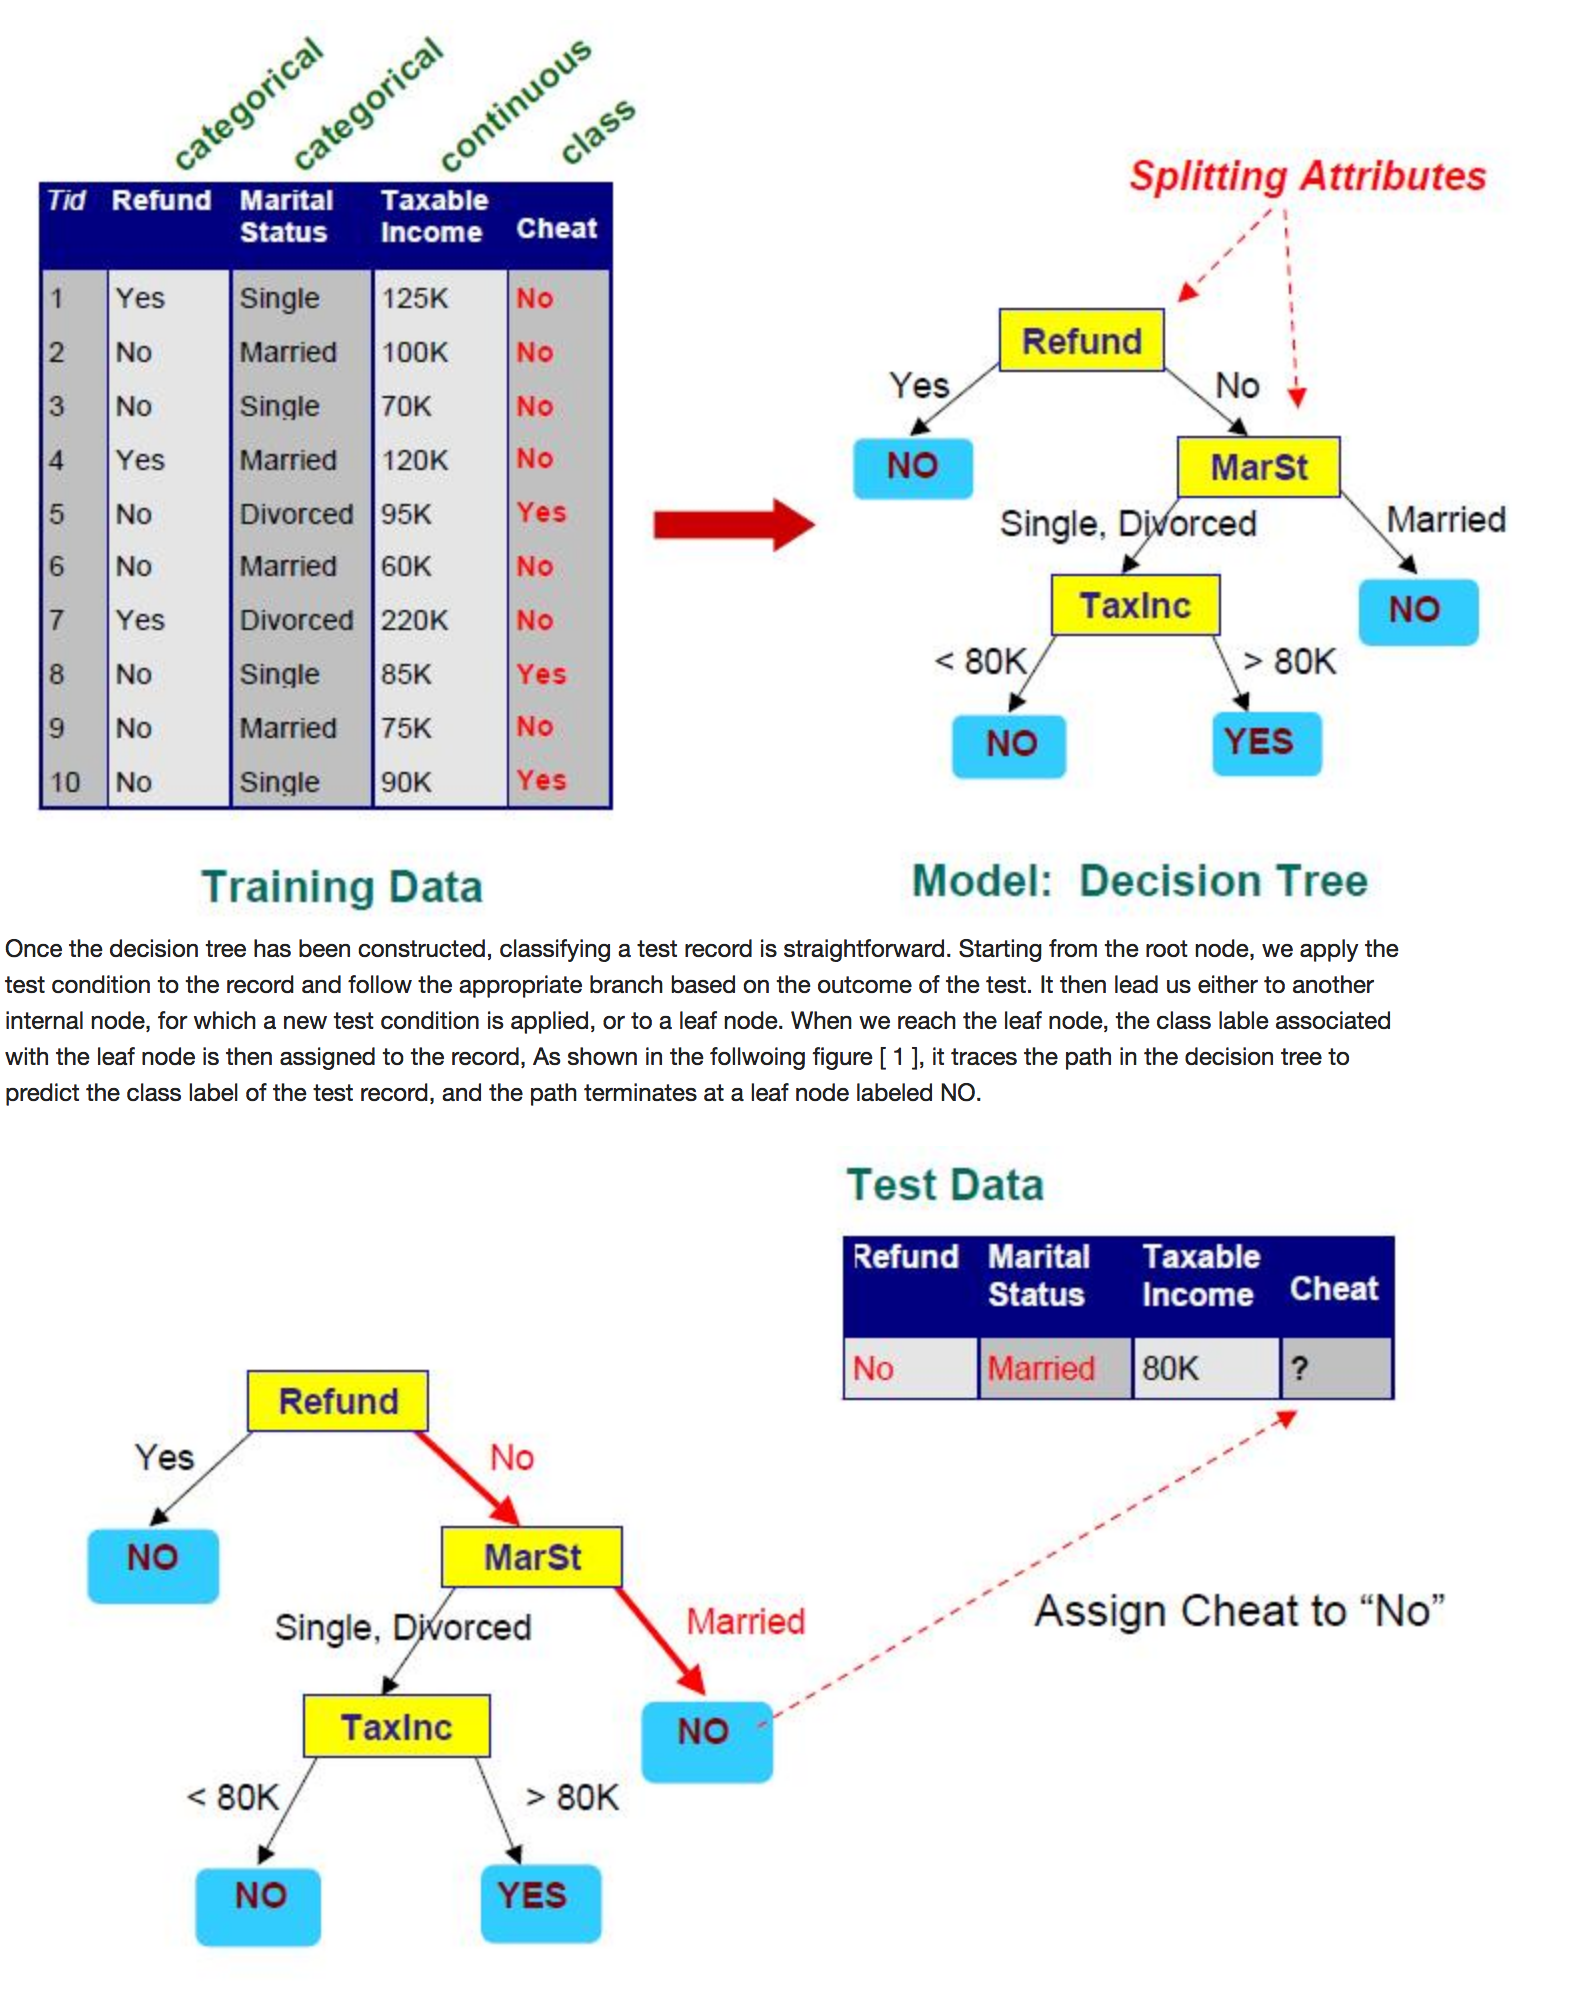
\includegraphics[width=0.6\textwidth]{DT-Example.png}
\end{center}
\end{frame}

\begin{frame}
\frametitle{How should we construct the tree?}
General process overview:
\begin{itemize}
\item Among all features, pick the one with most discriminative value (How?). \pause One approach: calculate "information gain" of all features and pick the one with highest gain. 
\item What is IG?: IG measures how much of a grouping can one feature do. How much reduction in "entropy" of the data (disorder) occurs due to this feature? \pause
\item What is entropy?: 
\begin{enumerate}
\item Entropy of a training dataset T is given by: \\ H(T) = $-\sum_{i=1}^c P(cat_i)log_2 P(cat_i)$ \\ where $P(cat_i)$ is the probability of getting $cat_i$ if you pick a random instance from training data.
\item If my training data has 9 instances of cat.A, 7 instances of cat.B, H(T) = $-[\frac{9}{16}log_2\frac{9}{16} + \frac{7}{16}log_2\frac{7}{16} ]$, which is 0.9836.
\end{enumerate}
\item What is the information gain of a feature? if T is the training data and f is a feature, IG(f) = H(T) - H(T$|$f) 
\end{itemize}
\end{frame}


\begin{frame}
\frametitle{How should we construct the tree? - intuition}
\begin{itemize}
\item The feature with the most IG splits the training data into some groups. Now, pick another feature which splits the data further. 
\item Keep organizing features that lets us split in a hierarchy like this, until no more splitting is possible and we end up with category labels at leaf nodes.
\pause 
\item Note of caution: I am oversimplifying. The actual training process involves more than this. Fortunately, you don't need to do all that yourself.
\item in NLTK: there is a class called DecisionTreeClassifier, which allows you to train and predict using decision trees.
\end{itemize}
\end{frame}

\begin{frame}
\frametitle{Random Forests}
\begin{itemize}
\item General idea: Combination of several classifiers will result in a better classifier ("bagging")
\item Random forests use decision trees for each of those "several" classifiers. \pause
\item Process:
\begin{enumerate}
\item Separate training data into some N datasets.
\item Build a decision tree with each of these N datasets (with all or some subset of features)
\item During prediction, use predictions from all the trees, and take a majority voting (or any such aggregation method) among all decision trees.
\item Same procedure can be used for numeric scale as well (average instead of majority in last step).
\end{enumerate} 
\item Generally considered robust. Can become slow with n-gram features as there are too many features. 
\end{itemize}
\end{frame}

%5min
\begin{frame}
\frametitle{Other Popular Algorithms}
\begin{itemize} 
\item Support Vector Machines
\item Neural network algorithms (aka "Deep Learning")
\item ... and many many more. If you really really want to know all details, take a machine learning course.
\item scikit-learn is a free machine learning library in Python that has implementations of several classification algorithms. \pause
\item Caution: scikit-learn, NLTK, or some other toolkit - each expect their input to be in a certain format. You should check their documentation about that, and write some code to convert data to the format these tools can understand.
\end{itemize}
\end{frame}

\begin{frame}
\frametitle{Assignment 4 Description}
\begin{itemize}
\item 2 questions, 15 marks (5+10)
\item for a change, no coding!!
\end{itemize}
\end{frame}

\begin{frame}
\frametitle{Next Class}
\begin{itemize}
\item Hui-Hsien's talk
\item Discussion about final projects
\item Text classification review and practice
\item Mid-term feedback
\end{itemize}
\end{frame}

\end{document}



